\documentclass{article}

% Required template
\usepackage[preprint]{colm2026_conference}

% Essential packages
\usepackage{amsmath,amsfonts,amssymb,amsthm}
\usepackage{graphicx}
\usepackage{booktabs}
\usepackage{hyperref}
\usepackage{xcolor}
\usepackage{tikz}
\usetikzlibrary{trees, shapes.geometric, arrows.meta, positioning, calc}
\usepackage{cleveref}
\usepackage{enumitem}

% Definitions and Macros
\newcommand{\E}{\mathbb{E}}
\newcommand{\KL}{D_{\mathrm{KL}}}
\newcommand{\ptheta}{P_\theta}
\newcommand{\pteacher}{P_{\mathcal{T}}}
\newcommand{\pdata}{P_{\mathrm{data}}}
\newcommand{\loss}{\mathcal{L}}

\title{On-Policy Distillation for Large Language Models: Methods, Systems, and Future Directions}

\author{
Anonymous Authors \\
\texttt{anonymous@domain.edu}
}

\begin{document}

\maketitle

\begin{abstract}
Knowledge distillation (KD) has historically served as the primary vehicle for model compression, transferring capabilities from massive teacher models to efficient student architectures. However, the advent of Large Language Models (LLMs) has catalyzed a fundamental paradigm shift from static, off-policy distillation to On-Policy Distillation (OPD). In this survey, we provide a comprehensive and theoretically grounded overview of OPD. We posit a core insight that must govern the modern understanding of distillation: the essence of OPD is not merely a choice of divergence metrics, but a profound paradigm shift in \textit{"who decides the training distribution."} By allowing the student's own generative manifold to dictate the state distribution, OPD directly mitigates the catastrophic train-test mismatch and compounding exposure bias inherent in autoregressive decoding. 
We systematically taxonomize the field into three converging trajectories based on feedback signals: Logit-based, Outcome-based, and Self-play methodologies. Furthermore, we critically analyze frequently neglected dimensions, including the compute-quality tradeoff, the teacher's "echo chamber" in uncertain regions, dynamic divergence adaptation, and the conceptualization of distillation as structured knowledge transfer rather than mere compression. Finally, we map out pivotal future directions, from distillation scaling laws to agent-level OPD.
\end{abstract}

\section{Introduction}
\label{sec:intro}

The evolution of Large Language Models (LLMs) has continuously pushed the boundaries of artificial intelligence, yet their massive parameter counts pose severe constraints on deployment and inference latency. Recently, the open-source community witnessed a monumental milestone: DeepSeek-R1 \citep{2501.12948} successfully distilled the profound reasoning capabilities of a 671B parameter Mixture-of-Experts (MoE) model into dense models as small as 7B parameters. This spectacular success underscores a vital reality—knowledge distillation is no longer a marginal optimization technique; it is the central engine for democratizing cutting-edge intelligence. The urgency to systematically understand and advance LLM distillation has never been greater.

Traditionally, distillation in Natural Language Processing has been heavily dominated by off-policy methods. In this paradigm, a student model is trained to mimic a teacher's token-level probabilities over a fixed, static dataset (i.e., $\pdata$). However, as elegantly illuminated by the "False Promise" of imitating proprietary LLMs \citep{2305.15717}, off-policy distillation suffers from a fatal, fundamental flaw: \textit{train-test mismatch}. During training, the student is conditioned on gold-standard prefixes from the dataset (teacher-forcing). During inference, the student must condition on its own previously generated tokens. When the student inevitably deviates from the optimal path, it enters out-of-distribution (OOD) territory where it has received no supervisory signal, leading to compounding errors—a phenomenon formally known as \textit{exposure bias}. 

To bridge this chasm, the field is rapidly migrating towards \textbf{On-Policy Distillation (OPD)}. Drawing deep conceptual linkages with Imitation Learning, specifically the DAgger (Dataset Aggregation) algorithm \citep{ross2011reduction}, OPD forces the student to generate trajectories according to its current policy ($\pi_\theta$), and selectively queries the teacher to provide feedback on these student-generated paths. 
\textbf{Core Insight 1:} \textit{The true essence of On-Policy Distillation is not simply the mathematical choice of probability divergence (e.g., Forward vs. Reverse KL), but rather a profound paradigm shift in "who decides the training distribution."} The shift from $y \sim \pdata$ to $y \sim \ptheta$ transforms the learning objective from memorizing an alien distribution to optimally navigating the student's own reachable generative manifold.

Despite the explosive growth of OPD methodologies—ranging from Generalized Knowledge Distillation (GKD) \citep{2306.13649} to MiniLLM \citep{2306.08543} and SPIN \citep{2401.01335}—the literature remains highly fragmented. Current surveys \citep{2402.13116} primarily treat distillation as a monolithic compression step, lacking a rigorous unified perspective on the on-policy dynamics. This paper addresses this critical gap. We dissect the mathematical foundations, categorize the emerging algorithmic variants, and spotlight the blind spots of current research.

Specifically, the contributions of this review are encapsulated in the following dimensions:
\begin{itemize}[leftmargin=*]
    \item \textbf{A Unified Theoretical Framework:} We rigorously formulate the transition from off-policy to on-policy distillation, mapping it directly to sequential decision-making and f-divergence minimization, mathematically unifying disparate works \citep{2306.13649, 2306.08543, 2402.03898}.
    \item \textbf{A Novel, Feedback-Centric Taxonomy:} We categorize the OPD landscape into three primary technical routes—\textit{Logit-based} (dense but requiring white-box access), \textit{Outcome-based} (sparse but highly flexible, utilizing Process Reward Models \citep{2305.20050}), and \textit{Self-play} (teacher-free but prone to saturation). We further highlight how these isolated tracks are actively converging, as seen in state-of-the-art frameworks like AlignDistil \citep{2503.02832} and MiMo-V2.
    \item \textbf{Identification of Neglected Critical Issues:} We bring to light fundamental challenges that the community has largely ignored: (a) The missing systematic analysis of the \textit{compute-quality tradeoff} in online distillation; (b) The "echo chamber" effect where querying teachers in regions of high student uncertainty leads to misaligned gradients; (c) The necessity for \textit{dynamic divergence} rather than static KL metric selection; and (d) Reconceptualizing distillation as \textit{structured knowledge transfer} rather than mere parameter compression.
    \item \textbf{Roadmap for Future Directions:} We chart the unexplored territories, detailing the necessity for distillation scaling laws, uncertainty-aware OPD, agent-level environmental distillation, and continuous distillation-RL loops.
\end{itemize}

The remainder of this paper is organized as follows. Section~\ref{sec:background} establishes the mathematical preliminaries, formalizing exposure bias and the f-divergence family. Section~\ref{sec:taxonomy} presents our novel taxonomy of OPD methodologies. [Note: Subsequent sections will cover detailed algorithmic analysis, fusion paradigms, critical challenges, and future directions.]


\section{Background and Preliminaries}
\label{sec:background}

To rigorously appreciate the leap from standard KD to On-Policy Distillation, we must first formalize the sequential nature of LLM generation and the mathematical definitions of distribution matching.

\subsection{Knowledge Distillation Fundamentals}
The classical Knowledge Distillation framework, pioneered by \cite{hinton2015distilling}, aims to transfer the "dark knowledge" (soft labels) from a teacher network $\mathcal{T}$ to a student network $\mathcal{S}$. For a given input $x$ and corresponding logits $z$, the probability distributions are smoothed by a temperature parameter $\tau > 0$:
\begin{equation}
    P(y|x; \tau) = \frac{\exp(z_y / \tau)}{\sum_{y'} \exp(z_{y'} / \tau)}
\end{equation}
The standard KD objective minimizes the Kullback-Leibler (KL) divergence between the teacher's softened distribution $\pteacher$ and the student's softened distribution $\ptheta$:
\begin{equation}
    \loss_{\mathrm{KD}} = \tau^2 \KL(\pteacher(\cdot|x; \tau) \parallel \ptheta(\cdot|x; \tau)) = \tau^2 \sum_{y} \pteacher(y|x; \tau) \log \left( \frac{\pteacher(y|x; \tau)}{\ptheta(y|x; \tau)} \right)
\end{equation}
The $\tau^2$ multiplier ensures the gradients scale appropriately relative to the standard cross-entropy loss.

\subsection{Token-Level vs Sequence-Level Distillation}
When extending KD to autoregressive language models, the sequence space $\mathcal{Y}$ grows exponentially with the sequence length $T$. As defined by \cite{kim2016sequence}, generation is parameterized as a product of conditional probabilities: $P(Y|X) = \prod_{t=1}^T P(y_t | y_{<t}, X)$.

\textbf{Token-Level KD (Word-Level KD):} The standard approach computes the divergence at each decoding step, strictly conditioned on the ground-truth prefix $y_{<t}^* \sim \pdata$:
\begin{equation}
    \loss_{\mathrm{Token-KD}} = \E_{X, Y^* \sim \pdata} \left[ \sum_{t=1}^{|Y^*|} \KL \left( \pteacher(y_t | y_{<t}^*, X) \parallel \ptheta(y_t | y_{<t}^*, X) \right) \right]
    \label{eq:token_kd}
\end{equation}

\textbf{Sequence-Level KD:} Conversely, sequence-level KD attempts to match the joint distribution over the entire trajectory:
\begin{equation}
    \loss_{\mathrm{Seq-KD}} = \E_{X \sim \pdata} \left[ \KL \left( \pteacher(Y|X) \parallel \ptheta(Y|X) \right) \right]
\end{equation}
Because the sum over all possible sequences $\sum_{Y \in \mathcal{Y}}$ is computationally intractable, off-policy Sequence-KD often relies on beam search to approximate the teacher's mode, generating a pseudo-dataset $\mathcal{D}_{\mathcal{T}}$, and performing standard maximum likelihood on this synthetic data.

\subsection{The Distribution Mismatch Problem and Exposure Bias}
Equation \ref{eq:token_kd} exposes the Achilles' heel of off-policy distillation. The expectation is taken over $Y^* \sim \pdata$, meaning the student only ever learns to predict the next token given a \textit{perfect} historical context. During inference, however, the student generates sequences auto-regressively: $\hat{y}_t \sim \ptheta(\cdot | \hat{y}_{<t}, X)$. 

If the student makes a slight error at step $t$, the context $\hat{y}_{\le t}$ diverges from the training support $\pdata$. Let $\epsilon$ be the probability of making a sub-optimal prediction at any time step. In standard supervised learning (off-policy), the error compounds quadratically. As demonstrated theoretically in Imitation Learning \citep{ross2011reduction}, an off-policy model traversing an $\epsilon$-suboptimal path for $T$ steps accumulates an error bounded by $\mathcal{O}(\epsilon T^2)$.

This compounding error, or \textit{exposure bias}, is precisely why models trained via standard KD on teacher outputs often hallucinate or structurally collapse during long-context reasoning \citep{2305.15717}. 

\subsection{The f-Divergence Family and Geometric Implications}
To address these issues, recent literature casts distillation as the minimization of an $f$-divergence \citep{2307.15190}. For two distributions $P$ and $Q$, the $f$-divergence is defined as:
\begin{equation}
    D_f(P \parallel Q) = \sum_{x} Q(x) f\left(\frac{P(x)}{Q(x)}\right)
\end{equation}
where $f$ is a convex function such that $f(1)=0$. The choice of $f$ dictates the geometric nature of the optimization, which profoundly impacts student behavior:

\textbf{1. Forward KL (Mode-Covering):} $f(t) = t \log t \implies D_{\mathrm{KL}}(\pteacher \parallel \ptheta)$. \\
Standard KD uses Forward KL. It severely penalizes $\ptheta(y) \to 0$ when $\pteacher(y) > 0$. Consequently, the student tries to cover all modes of the teacher. If the student lacks the capacity to capture a highly multimodal teacher distribution, it will average across modes, assigning probability mass to regions of the space where $\pteacher = 0$ (generating gibberish).

\textbf{2. Reverse KL (Mode-Seeking):} $f(t) = -\log t \implies D_{\mathrm{KL}}(\ptheta \parallel \pteacher)$. \\
Utilized by MiniLLM \citep{2306.08543}, Reverse KL penalizes $\ptheta(y) > 0$ when $\pteacher(y) \to 0$ (zero-forcing). The student seeks out the single dominant mode of the teacher and ignores the rest. This encourages highly confident, coherent, and safe text generation, effectively pruning invalid reasoning paths.

\textbf{3. Jensen-Shannon Divergence (JSD):} Utilized by GKD \citep{2306.13649}, JSD provides a symmetric compromise, interpolating between mode-covering and mode-seeking behaviors.

\textbf{Dynamic Divergence:} A neglected core insight is that the optimal divergence is not static. A student might require mode-covering during early training phases to explore the vocabulary space, and mode-seeking in later stages to refine complex reasoning trajectories.

\subsection{From Off-Policy to On-Policy: A Unified View}
\label{sec:unified_view}

The transition to On-Policy Distillation fundamentally alters the expectation distribution. We unify approaches like GKD \citep{2306.13649}, MiniLLM \citep{2306.08543}, and DistiLLM \citep{2402.03898} under the following continuous formulation:
\begin{equation}
    \loss_{\mathrm{OPD}} = \E_{X \sim \pdata} \left[ \E_{Y \sim \ptheta(\cdot|X)} \left[ \sum_{t=1}^{|Y|} D_f \left( \pteacher(\cdot | Y_{<t}, X) \parallel \ptheta(\cdot | Y_{<t}, X) \right) \right] \right]
\end{equation}

Here, the expectation over sequences $Y$ is drawn from the \textbf{student's current policy} $\ptheta$, not the fixed dataset $\pdata$. 
By actively rolling out the student policy $\hat{y}_{<t} \sim \ptheta$, the student explores its own sub-optimal manifold. The teacher $\pteacher$ then provides an oracle correction $\pteacher(\cdot | \hat{y}_{<t}, X)$ on this specific, potentially drifted state. This formulation strictly bounds the sequential error to $\mathcal{O}(\epsilon T)$ \citep{ross2011reduction}, directly solving exposure bias. Thus, the essence of OPD is a pedagogical shift: instead of forcing the student to walk the teacher's exact footsteps, the teacher observes where the student naturally walks and guides its next step from there.

\section{Taxonomy of On-Policy Distillation}
\label{sec:taxonomy}

As the field of On-Policy Distillation expands, methodologies have proliferated with different assumptions regarding teacher access, feedback types, and optimization algorithms. To provide structured clarity, we present a novel taxonomy primarily organized by the \textit{source and nature of the feedback signal}. \Cref{fig:taxonomy} illustrates this hierarchical categorization.

\begin{figure}[htbp]
\centering
\resizebox{\textwidth}{!}{%
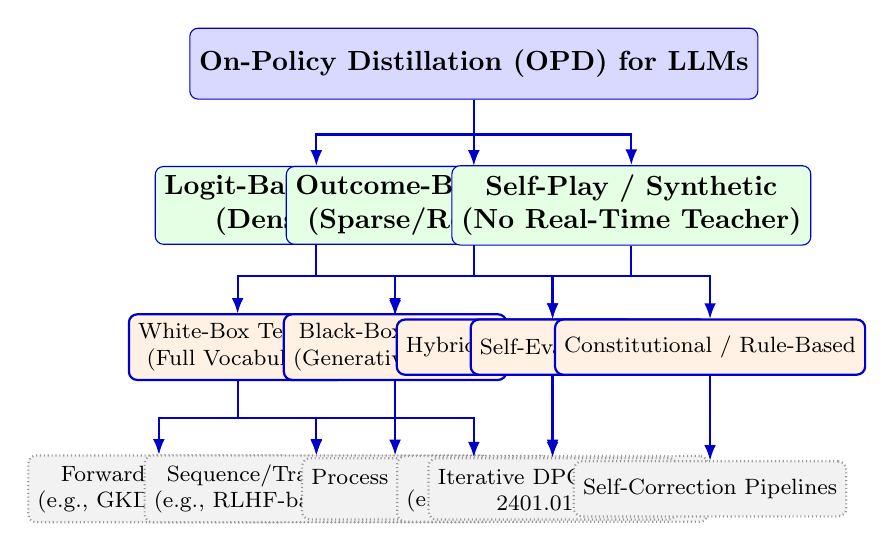
\begin{tikzpicture}[
    level distance=1.8cm,
    sibling distance=2cm,
    every node/.style={rectangle, draw=blue!80!black, rounded corners=3pt, align=center, fill=blue!5, font=\footnotesize, minimum height=0.7cm},
    edge from parent fork down,
    edge from parent/.style={draw, -{Latex[length=2mm, width=1.5mm]}, thick, blue!80!black},
    root/.style={fill=blue!15, font=\normalsize\bfseries, minimum height=0.9cm},
    lvl1/.style={fill=green!10, font=\bfseries},
    lvl2/.style={fill=orange!10},
    lvl3/.style={fill=gray!10, draw=gray!80, densely dotted}
]

% Root Node
\node[root] (Root) {On-Policy Distillation (OPD) for LLMs}
    % Branch 1: Logit-based
    child {node[lvl1] {Logit-Based Feedback\\(Dense Signal)}
        child {node[lvl2] {White-Box Teacher\\(Full Vocabulary)}
            child {node[lvl3] {Forward KL / JSD\\(e.g., GKD \citep{2306.13649})}}
            child {node[lvl3] {Reverse KL\\(e.g., MiniLLM \citep{2306.08543})}}
        }
        child {node[lvl2] {Restricted / Top-$K$\\Teacher Access}
            child {node[lvl3] {Truncated f-Divergence\\(e.g., DistiLLM \citep{2402.03898})}}
        }
    }
    % Branch 2: Outcome-based
    child {node[lvl1] {Outcome-Based Feedback\\(Sparse/Reward Signal)}
        child {node[lvl2] {Black-Box Teacher\\(Generative Oracle)}
            child {node[lvl3] {Sequence/Trajectory Reward\\(e.g., RLHF-based KD, RLKD)}}
            child {node[lvl3] {Process Reward Models (PRM)\\ \citep{2305.20050}}}
        }
        child {node[lvl2] {Hybrid / Fusion Approaches}
            child {node[lvl3] {Logit + Reward Fusion\\(e.g., MiMo-V2, AlignDistil)}}
        }
    }
    % Branch 3: Self-play
    child {node[lvl1] {Self-Play / Synthetic\\(No Real-Time Teacher)}
        child {node[lvl2] {Self-Evaluator}
            child {node[lvl3] {Iterative DPO / SPIN\\ \citep{2401.01335}}}
        }
        child {node[lvl2] {Constitutional / Rule-Based}
            child {node[lvl3] {Self-Correction Pipelines}}
        }
    };

\end{tikzpicture}
}
\caption{Taxonomy of On-Policy Distillation methods for Large Language Models. Our classification maps the paradigm across three distinct feedback signals, detailing the varying degrees of teacher visibility and optimization granularity. Crucially, contemporary methods are increasingly blurring the lines between these branches via Hybrid Fusion approaches.}
\label{fig:taxonomy}
\end{figure}

Our taxonomy reveals three dominant trajectories:

\textbf{1. Logit-Based Feedback (Dense, White-Box):} 
This branch operates on the traditional premise of KD, requiring access to the teacher's probability distribution over the vocabulary. Because feedback is provided at the token level ($t=1 \dots T$), the supervisory signal is extremely dense. Methods here are sub-categorized by divergence choice and teacher access constraints. GKD \citep{2306.13649} utilizes Forward KL and JSD on student-generated prefixes. MiniLLM \citep{2306.08543} leverages the REINFORCE algorithm to optimize Reverse KL, encouraging mode-seeking behavior. However, computing full-vocabulary logits from massive teachers (e.g., GPT-4) is often impossible due to API restrictions. Consequently, methods like DistiLLM \citep{2402.03898} adapt these losses to operate strictly on the Top-$K$ logits returned by black-box APIs, interpolating between hard-label matching and full-distribution mimicking.

\textbf{2. Outcome-Based Feedback (Sparse, Black-Box):} 
When logit access is completely restricted, or when distilling complex reasoning tasks (e.g., mathematics, coding), the field shifts to Outcome-Based Feedback. Here, the student generates full or partial trajectories, and the teacher (or a proxy reward model derived from the teacher) scores the sequence. This approach relies heavily on Reinforcement Learning paradigms (e.g., PPO, GRPO). The integration of Process Reward Models (PRMs) \citep{2305.20050} has been revolutionary in this space, allowing the sparse sequence-level reward to be decomposed into step-by-step reasoning feedback, maintaining the flexibility of black-box distillation while mitigating the sparsity of the signal.

\textbf{3. Self-Play and Synthetic Paradigms (Teacher-Free):} 
A radical departure from standard distillation is the elimination of the active external teacher during the on-policy loop. In methods like SPIN (Self-Play Fine-Tuning) \citep{2401.01335}, the student plays a min-max game against its own historical checkpoints. By treating the initial off-policy distilled dataset as the "expert," the student continuously generates responses on-policy and contrasts them via DPO (Direct Preference Optimization) against the expert data. While highly scalable, this route heavily risks capability saturation, as no new external knowledge is introduced into the system.

\textbf{The Convergence of Trajectories:} 
\textbf{Core Insight 2:} \textit{The boundaries between these three routes are rapidly dissolving.} State-of-the-art frameworks represent a fusion of these paradigms. For instance, AlignDistil \citep{2503.02832} unifies alignment (Outcome-based RL) and distillation (Logit-based) into a single cohesive objective, demonstrating that matching teacher distributions and maximizing downstream human-preference rewards are intrinsically complementary. Similarly, emerging architectures like MiMo-V2 blend multi-teacher logit ensembles with token-level reward signals to guide on-policy exploration. This taxonomy underscores that future breakthroughs will likely emerge not from isolated branches, but from the strategic hybridization of dense logit feedback with sparse, outcome-driven environmental exploration.

\end{document}
